\documentclass{beamer}
\usetheme{DarkConsole}
\usepackage{circuitikz}
\usetikzlibrary{arrows}
%\usepackage{enumitem}
\usepackage{cmtt}
\usetikzlibrary{positioning}


\definecolor{bitcoinorange}{RGB}{255,165,0}

% Define a subcircuit 'divider' with input and output
\ctikzsubcircuitdef{divider}{in, out}{%
  coordinate (#1-in) to[R, l=$Z_s$, name=#1-rh, -*] ++(2,0)
  coordinate(#1-tmp) to[R, l=$Z_L$, name=#1-rl] ++(0,-2)
  node[tlground]{} (#1-tmp) --++(0.5,0) coordinate(#1-out)
}

% Define a custom command to use the 'divider' subcircuit
\newcommand{\mydiv}[4]{
  \divider{#1}{#2} (#1-rh.n) node[above] {$#3$}
  (#1-rl.n) node[right] {$#4$} (#1-out)
}


% Title page information
\title{Self Sovereign Communications Infrastructure?}
\author{Chandran}
% \date{\today}
\date{September 29, 2023}

\begin{document}

\begin{frame}

  \begin{tikzpicture}[remember picture,overlay]
    \draw ([yshift=-0.8cm,xshift=-2.9cm]current page.north east) \mydiv{a}{in}{}{};
  \end{tikzpicture}

  \titlepage
\end{frame}


\begin{frame}{Outline}

  \begin{tikzpicture}[remember picture,overlay]
    \draw ([yshift=-0.8cm,xshift=-2.9cm]current page.north east) \mydiv{a}{in}{}{};
  \end{tikzpicture}

    \tableofcontents

\end{frame}

\section{Infrastructure Tree}

\begin{frame}{Introduction}

  \begin{tikzpicture}[remember picture,overlay]
    \draw ([yshift=-0.8cm,xshift=-2.9cm]current page.north east) \mydiv{a}{in}{}{};
  \end{tikzpicture}

  \begin{minipage}[t]{0.5\textwidth} % Adjust the width as needed
\begin{figure}
  \centering
  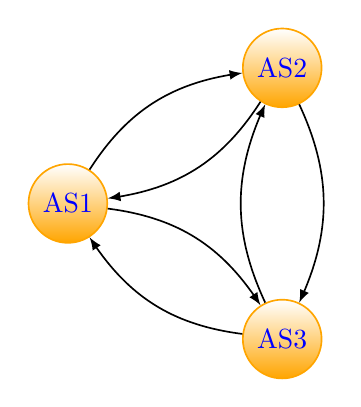
\begin{tikzpicture}[-latex, auto, node distance=1cm and 2cm, semithick,
    state/.style={circle, top color=white, bottom color=bitcoinorange,
    draw=bitcoinorange, text=blue, minimum width=1cm}]

    \node[state] (AS1) {AS1};
    \node[state] (AS2) [above right=of AS1] {AS2};
    \node[state] (AS3) [below right=of AS1] {AS3};

    \path (AS1) edge [bend left=25] node[above] {} (AS2);
    \path (AS2) edge [bend left=25] node[below] {} (AS1);

    \path (AS1) edge [bend left=25] node[above] {} (AS3);
    \path (AS3) edge [bend left=25] node[below] {} (AS1);

    \path (AS2) edge [bend left=25] node[above] {} (AS3);
    \path (AS3) edge [bend left=25] node[below] {} (AS2);
  \end{tikzpicture}
  \caption{Internet as Autonomous Systems (AS) in a \textbf{flat hierarchy}}
\end{figure}
  \end{minipage}%
  \begin{minipage}[t]{0.5\textwidth} % Adjust the width as needed

Test bla bla

  \end{minipage}%

\end{frame}

\section{Tradeoffs}


\begin{frame}{Introduction}

  \begin{tikzpicture}[remember picture,overlay]
    \draw ([yshift=-0.8cm,xshift=-2.9cm]current page.north east) \mydiv{a}{in}{}{};
  \end{tikzpicture}

    \vspace{-2cm} % Adjust the vertical space as needed

  \begin{minipage}[t]{0.5\textwidth} % Adjust the width as needed
    \setlength{\parskip}{10pt} % Adjust the value to increase or decrease space
    \tableofcontents
  \end{minipage}%
  \begin{minipage}[t]{0.5\textwidth} % Adjust the width as needed
    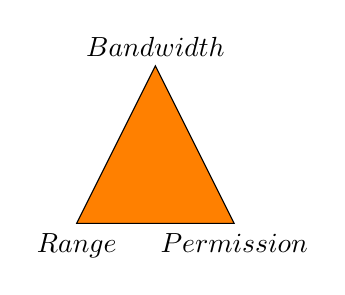
\begin{tikzpicture}
      % Define triangle coordinates
      \coordinate (A) at (0,0);
      \coordinate (B) at (2,0);
      \coordinate (C) at (1,2);

      % Draw the isosceles triangle
      \draw[fill=orange] (A) -- (B) -- (C) -- cycle;

      % Label the corners
      \node[below] at (A) {$Range$};
      \node[below] at (B) {$Permission$};
      \node[above] at (C) {$Bandwidth$};
    \end{tikzpicture}
  \end{minipage}


\end{frame}


\section{Message Value and Cost}

\begin{frame}{Main Content}
  \begin{tikzpicture}[remember picture,overlay]
    \draw ([yshift=-0.8cm,xshift=-2.9cm]current page.north east) \mydiv{a}{in}{}{};
  \end{tikzpicture}

  \begin{itemize}
    \item Bullet point 1
    \item Bullet point 2
    \item Bullet point 3
  \end{itemize}
\end{frame}

\begin{frame}{What next?}

  \begin{tikzpicture}[remember picture,overlay]
    \draw ([yshift=-0.8cm,xshift=-2.9cm]current page.north east) \mydiv{a}{in}{}{};
  \end{tikzpicture}

  \begin{enumerate}
    \item Item 1
    \item Item 2
    \item Item 3
  \end{enumerate}
\end{frame}

\section{What next?}

\begin{frame}{Conclusion}

  \begin{tikzpicture}[remember picture,overlay]
    \draw ([yshift=-0.8cm,xshift=-2.9cm]current page.north east) \mydiv{a}{in}{}{};
  \end{tikzpicture}

  This is the conclusion slide.
\end{frame}

\begin{frame}{Thank You}

  \begin{tikzpicture}[remember picture,overlay]
    \draw ([yshift=-0.8cm,xshift=-2.9cm]current page.north east) \mydiv{a}{in}{}{};
  \end{tikzpicture}

  \centering
  \Huge Thank you for your attention!
\end{frame}

\end{document}
